\documentclass[tikz, margin=2mm]{standalone}
\usepackage[utf8]{inputenc}
\usepackage{tikz}
\usetikzlibrary{matrix,backgrounds,positioning}

\begin{document}
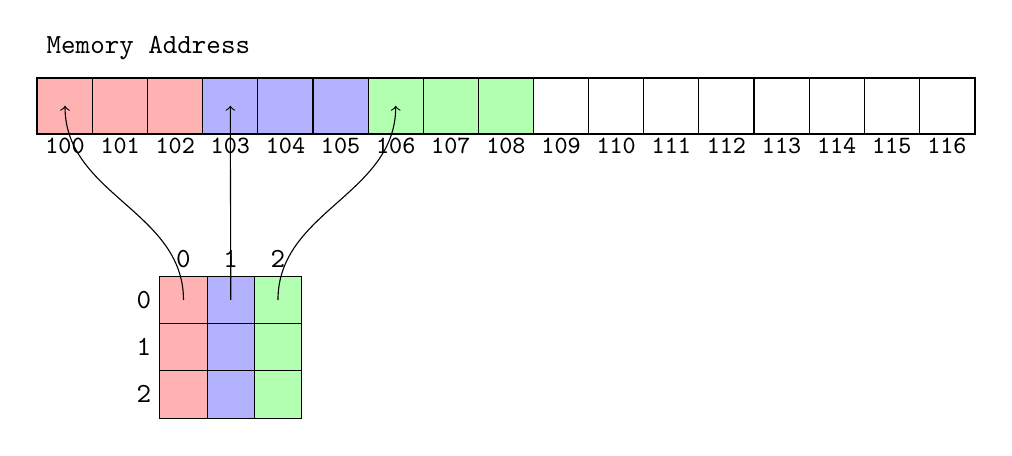
\begin{tikzpicture}[%
    arraynode/.style={
        draw,
        node contents={[\the\numexpr\pgfmatrixcurrentrow-2\relax][\the\numexpr\pgfmatrixcurrentcolumn-2\relax]},
        alias=n\the\numexpr\pgfmatrixcurrentrow-2\relax\the\numexpr\pgfmatrixcurrentcolumn-2\relax
        },
    columnlabel/.style={
        minimum size=0pt,
        draw=none,
        red,
        node contents={\the\numexpr\pgfmatrixcurrentcolumn-2\relax},
        alias=c\the\numexpr\pgfmatrixcurrentcolumn-2\relax
        },      
    rowlabel/.style={
        minimum size=0pt,
        draw=none,
        red,
        node contents={\the\numexpr\pgfmatrixcurrentrow-2\relax},
        alias=r\the\numexpr\pgfmatrixcurrentrow-2\relax
        },      
    emptynode/.style={node contents=~, draw=none},
    font=\ttfamily,
    array/.style={%
        matrix of nodes,
        nodes = arraynode,
        column sep=-\pgflinewidth,
        row sep=-\pgflinewidth, 
        nodes in empty cells,
        row 1/.style={nodes=columnlabel},
        column 1/.style={nodes=rowlabel},
        row 1 column 1/.style={%
            nodes=emptynode}}, 
    rowlabel2/.style={
        inner sep=2pt,
        draw=none,
        font=\small\ttfamily,
        node contents={\the\numexpr99+\pgfmatrixcurrentcolumn\relax},
        alias=m\the\numexpr99+\pgfmatrixcurrentcolumn\relax
        },      
    memoryrow/.style={%
        matrix of nodes,
        row 1/.style={nodes = {draw, minimum size=7mm}},
        column sep=-\pgflinewidth,
        row sep=-\pgflinewidth, 
        nodes in empty cells,
        row 2/.style={nodes=rowlabel2}}, 
    memory/.style={%
        matrix of nodes,
        nodes={draw, minimum size=6mm, anchor=center},
        row 1/.style={nodes = {columnlabel, black}},
        column 1/.style={nodes = {rowlabel, black}},
        row 1 column 1/.style={nodes = emptynode},
        column sep=-\pgflinewidth,
        row sep=-\pgflinewidth, 
        nodes in empty cells,
    } 
]

%\matrix[array] (array) {
%&&&&\\
%&&&&\\
%&&&&\\
%&&&&\\};

%\node[above= 4mm of n01.north east] {Columns};
%\node[left= 0mm of r1, rotate=90, anchor=south] {Rows};
%\draw[<-] (c0.west)--++(130:1cm) node[above, draw]{2nd subscript};
%\draw[<-] (r2.south)--++(250:1cm) node[below, draw]{1st subscript};
%\draw[<-] ([shift={(-1mm,-1mm)}]n02.north east)--++(65:2cm) node[above, draw, text width=3cm]{Element's subscript order};

\begin{scope}[yshift=-4cm]

\matrix[memoryrow] (memrow) {
&&&&&&&&&&&&&&&&\\
&&&&&&&&&&&&&&&&\\};

\node[above right=1mm and 0 of memrow-1-1.north west] {Memory Address};
%\node[above right=1mm and 0 of memrow-1-1.north west] {Memory Address};
\draw[thick] (memrow-1-1.north west) rectangle (memrow-1-17.south east);

\matrix[memory, below left=8mm and -11.5mm of memrow, anchor=north west] (memory) {
&&&\\
&&&\\
&&&\\
&&&\\};

\begin{scope}[on background layer]
\fill[red!30] (memrow-1-1.north west) rectangle (memrow-1-3.south east);
\fill[blue!30] (memrow-1-4.north west) rectangle (memrow-1-6.south east);
\fill[green!30] (memrow-1-7.north west) rectangle (memrow-1-9.south east);

\fill[red!30] (memory-2-2.north west) rectangle (memory-4-2.south east);
\fill[blue!30] (memory-2-3.north west) rectangle (memory-4-3.south east);
\fill[green!30] (memory-2-4.north west) rectangle (memory-4-4.south east);


\end{scope}
\draw[->] (memory-2-2.center) to[out=90, in=-90] (memrow-1-1.center);
\draw[->] (memory-2-3.center) to[out=90, in=-90] (memrow-1-4.center);
\draw[->] (memory-2-4.center) to[out=90, in=-90] (memrow-1-7.center);
\end{scope}

\end{tikzpicture}
\end{document}